% !TEX TS-program = pdflatexmk
\documentclass[12pt]{article}

% Layout.
\usepackage[top=1in, bottom=0.75in, left=1in, right=1in, headheight=1in, headsep=6pt]{geometry}

% Fonts.
\usepackage{mathptmx}
\usepackage[scaled=0.86]{helvet}
\renewcommand{\emph}[1]{\textsf{\textbf{#1}}}
\newcommand{\ans}[1][1in]{\rule{#1}{.5pt}}

\usepackage[parfill]{parskip}

% Misc packages.
\usepackage{amsmath,amssymb,latexsym}
\usepackage{graphicx,hyperref}
\usepackage{array}
\usepackage{xcolor}
\usepackage{multicol,tikz}
\usepackage{tabularx,colortbl,booktabs,xparse}
\usepackage{enumitem}

% Rotation: \rot[<angle>][<width>]{<stuff>}
\NewDocumentCommand{\rot}{O{45} O{1em} m}{\makebox[#2][l]{\rotatebox{#1}{#3}}}%

\usepackage{fancyhdr}
\pagestyle{fancy} 
\lhead{\large\sf\textbf{MATH F113X: Eulerization}}
%\chead{\large\sf\textbf{lecture notes}}
%\rhead{\large\sf\textbf{Day 1}}

\begin{document}

The goals are to understand:
\begin{itemize}
\item how to Eulerize a graph
\item why you would Eulerize a graph
\item how to put Dijkstra's algorithm together with Euler circuits
\end{itemize}
\begin{enumerate}
\item Recall problem 5 from Worksheet 12:
\begin{quote}
Add (the fewest number of) edges to the graph below in order to force every vertex to have even degree. Then find an Euler circuit in the resulting graph.\\

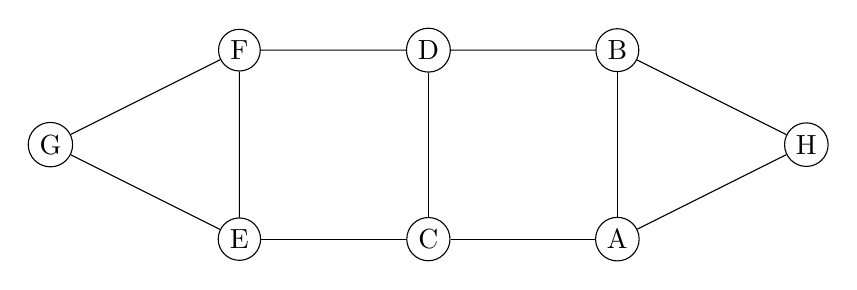
\begin{tikzpicture}[baseline=(current bounding box.center), scale=.8]
\tikzstyle{every node}=[circle, draw, fill=black!0,
                        inner sep=2pt, minimum width=10pt]
\path (0,0) node (A) {A} ;
\node (B)  at (-0,3) {B};
\node (C) at (-3,0) {C} ;
\node (E) at (-6,0) {E} ;
\node (F) at (-6,3)  {F} ;
\node (D) at (-3,3)  {D};
\node (G) at (-9, 1.5) {G};
\node (H) at (3,1.5) {H};
\foreach \i/\j in {A/B,B/D,A/C, C/D, C/E,E/F,A/H,B/H, D/F,G/F, G/E}{\draw (\i) -- (\j);}
\end{tikzpicture}
\end{quote}
\quad\\
\hrule

\quad\\
 Below are several answers from the worksheet. What do you observe?\\
 
\begin{tabularx}{\textwidth}{XX}
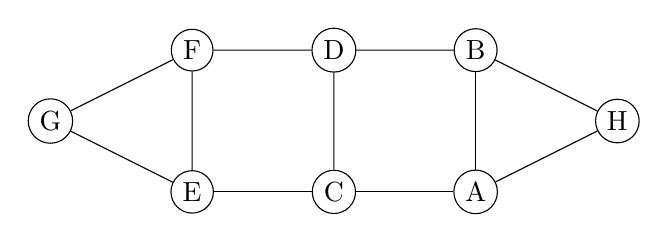
\begin{tikzpicture}[baseline=(current bounding box.center), scale=.6]
\tikzstyle{every node}=[circle, draw, fill=black!0,
                        inner sep=2pt, minimum width=10pt]
\path (0,0) node (A) {A} ;
\node (B)  at (-0,3) {B};
\node (C) at (-3,0) {C} ;
\node (E) at (-6,0) {E} ;
\node (F) at (-6,3)  {F} ;
\node (D) at (-3,3)  {D};
\node (G) at (-9, 1.5) {G};
\node (H) at (3,1.5) {H};
\foreach \i/\j in {A/B,B/D,A/C, C/D, C/E,E/F,A/H,B/H, D/F,G/F, G/E}{\draw (\i) -- (\j);}
\end{tikzpicture}
&
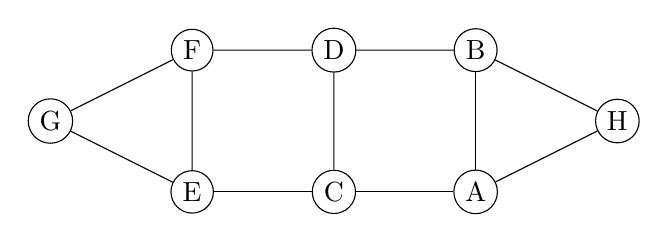
\begin{tikzpicture}[baseline=(current bounding box.center), scale=.6]
\tikzstyle{every node}=[circle, draw, fill=black!0,
                        inner sep=2pt, minimum width=10pt]
\path (0,0) node (A) {A} ;
\node (B)  at (-0,3) {B};
\node (C) at (-3,0) {C} ;
\node (E) at (-6,0) {E} ;
\node (F) at (-6,3)  {F} ;
\node (D) at (-3,3)  {D};
\node (G) at (-9, 1.5) {G};
\node (H) at (3,1.5) {H};
\foreach \i/\j in {A/B,B/D,A/C, C/D, C/E,E/F,A/H,B/H, D/F,G/F, G/E}{\draw (\i) -- (\j);}
\end{tikzpicture}
\end{tabularx}
\vfill

\begin{tabularx}{\textwidth}{XX}
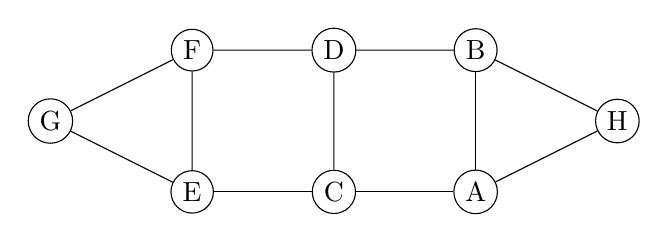
\begin{tikzpicture}[baseline=(current bounding box.center), scale=.6]
\tikzstyle{every node}=[circle, draw, fill=black!0,
                        inner sep=2pt, minimum width=10pt]
\path (0,0) node (A) {A} ;
\node (B)  at (-0,3) {B};
\node (C) at (-3,0) {C} ;
\node (E) at (-6,0) {E} ;
\node (F) at (-6,3)  {F} ;
\node (D) at (-3,3)  {D};
\node (G) at (-9, 1.5) {G};
\node (H) at (3,1.5) {H};
\foreach \i/\j in {A/B,B/D,A/C, C/D, C/E,E/F,A/H,B/H, D/F,G/F, G/E}{\draw (\i) -- (\j);}
\end{tikzpicture}
&
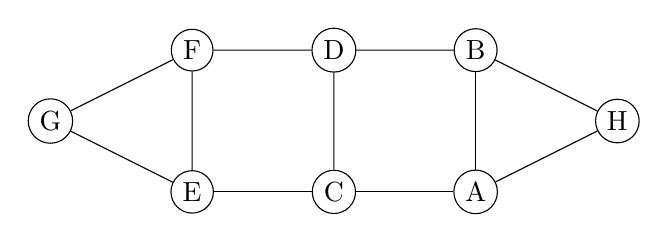
\begin{tikzpicture}[baseline=(current bounding box.center), scale=.6]
\tikzstyle{every node}=[circle, draw, fill=black!0,
                        inner sep=2pt, minimum width=10pt]
\path (0,0) node (A) {A} ;
\node (B)  at (-0,3) {B};
\node (C) at (-3,0) {C} ;
\node (E) at (-6,0) {E} ;
\node (F) at (-6,3)  {F} ;
\node (D) at (-3,3)  {D};
\node (G) at (-9, 1.5) {G};
\node (H) at (3,1.5) {H};
\foreach \i/\j in {A/B,B/D,A/C, C/D, C/E,E/F,A/H,B/H, D/F,G/F, G/E}{\draw (\i) -- (\j);}
\end{tikzpicture}
\end{tabularx}
\vfill
\begin{tabularx}{\textwidth}{XX}
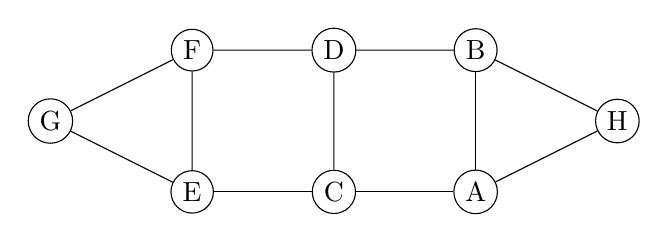
\begin{tikzpicture}[baseline=(current bounding box.center), scale=.6]
\tikzstyle{every node}=[circle, draw, fill=black!0,
                        inner sep=2pt, minimum width=10pt]
\path (0,0) node (A) {A} ;
\node (B)  at (-0,3) {B};
\node (C) at (-3,0) {C} ;
\node (E) at (-6,0) {E} ;
\node (F) at (-6,3)  {F} ;
\node (D) at (-3,3)  {D};
\node (G) at (-9, 1.5) {G};
\node (H) at (3,1.5) {H};
\foreach \i/\j in {A/B,B/D,A/C, C/D, C/E,E/F,A/H,B/H, D/F,G/F, G/E}{\draw (\i) -- (\j);}
\end{tikzpicture}
&
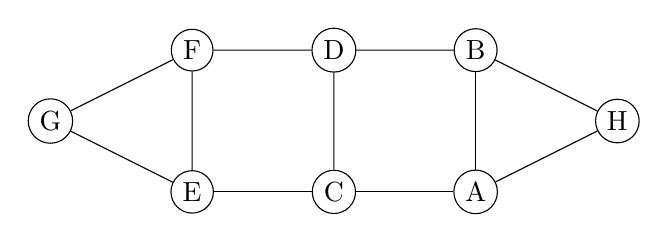
\begin{tikzpicture}[baseline=(current bounding box.center), scale=.6]
\tikzstyle{every node}=[circle, draw, fill=black!0,
                        inner sep=2pt, minimum width=10pt]
\path (0,0) node (A) {A} ;
\node (B)  at (-0,3) {B};
\node (C) at (-3,0) {C} ;
\node (E) at (-6,0) {E} ;
\node (F) at (-6,3)  {F} ;
\node (D) at (-3,3)  {D};
\node (G) at (-9, 1.5) {G};
\node (H) at (3,1.5) {H};
\foreach \i/\j in {A/B,B/D,A/C, C/D, C/E,E/F,A/H,B/H, D/F,G/F, G/E}{\draw (\i) -- (\j);}
\end{tikzpicture}
\end{tabularx}
\vfill
\newpage
\item \textbf{Definition:} To \textbf{eulerize} a graph $G$ means\\

\vfill

\item \textbf{Definition:} An \textbf{optimal eulerization} means \\

\vfill

\item Under what conditions do you think it is \textit{easy} to obtain an optimal eulerization?

\vfill

\end{enumerate}
\end{document}